%%%%%%%%%%%%%%%%%%%%%%%%%%%%%%%%%%%%%%%%%%%%%%%%%%%%%%%%%%%%%%%%%%%%%%%%
% Golden Sacra - Memoria
% Escuela Politécnica Superior de la Universidad de Alicante
% Realizado por: Ángel Jesús Terol Martínez
% Contacto: jtm37@alu.ua.es
%%%%%%%%%%%%%%%%%%%%%%%%%%%%%%%%%%%%%%%%%%%%%%%%%%%%%%%%%%%%%%%%%%%%%%%%
\chapter{Game Design Document}
\label{gdd}

\section{Características}

\begin{itemize}
	\item \textbf{Título:} Golden Sacra
	\item \textbf{Plataforma:} Game Boy - Game Boy Color
	\item \textbf{Género:} Aventuras, RPG/Nethack
	\item \textbf{Idioma:} Inglés
	\item \textbf{Público Objetivo:} Cualquier persona mayor de 3 años.
\end{itemize}

\section{Historia}

La historia transcurre en una \textbf{pequeña aldea} conocida como \textit{Elry}. La vida es tranquila y plácida, menos para \textbf{nuestra protagonista Ashia}, cuyo \textbf{padre} padece de una \textbf{enfermedad extraña} y su cura procede únicamente de una planta llamada \textit{Inis}. Este tipo de plantas solamente crecen en las profundidades de las mazmorras más inhóspitas y terroríficas que un humano pueda pisar.
\\ \\
Sin llegar a ver mejoría alguna en su padre y que ninguna persona cercana podía proporcionarles el susodicho remedio, \textbf{decidió adentrarse en las cuevas cercanas con el objetivo de encontrarlo}. Sin experiencia de combate, lo único que la acompañaba era el valor.

\section{Mecánicas}

Para avanzar en \textit{Golden Sacra}, deberemos adentrarnos en las distintas mazmorras y \textbf{llegar hasta el piso más profundo} de todos. Para ello, el jugador deberá ir derrotando a los enemigos que le corten el paso y encontrar las escaleras que le conduzcan al siguiente piso.

\clearpage

\begin{figure}[h]
\centering
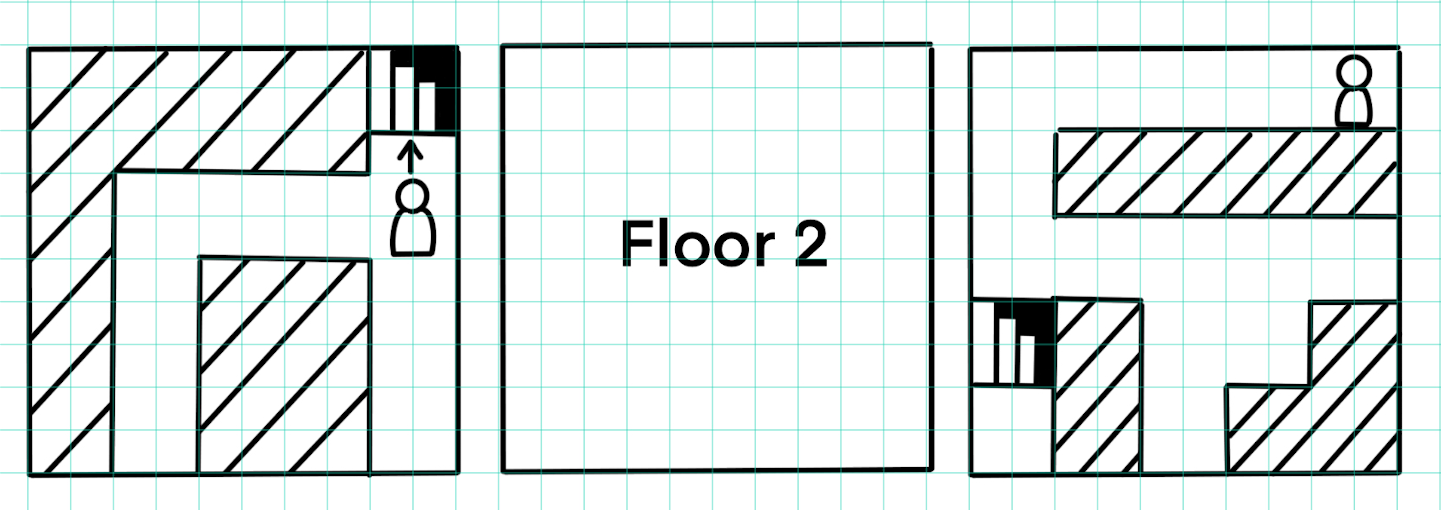
\includegraphics[width=0.9\textwidth]{include/images/gdd/gdd_floors.png}
\caption{Mockup - Avance de Juego}
\label{figure:protagonist}
\end{figure}

El movimiento y el sistema de combate funcionan por \textbf{turnos}. El primer turno será para el jugador, donde podrá decidir entre las acciones de moverse, atacar o utilizar un objeto, para luego dar paso al turno de los enemigos. \textbf{No todas las acciones consumen el turno}: cambiar el equipamiento, cambiar la dirección en la que el personaje mira, etc.
\\ \\
El jugador dispondrá de un valor de hambre,el cual irá disminuyendo conforme gastemos nuestro turno. Si la barra llega a 0, \textbf{por cada turno la vida irá disminuyendo}. Para evitar que esto ocurra, deberá encontrar objetos que pueda comer para satisfacerse. En el HUD no se dispondrá de una barra de hambre, equivalente a la que habrá con la vida. Conforme el hambre disminuya, llegados a un punto saldrán dos mensajes de advertencia: un primer mensaje para cuando está por debajo del 20\%, y otro para cuando ha llegado al 0\% (teniendo en cuenta que no tener nada de hambre es un valor del 100\%).

\begin{figure}[h]
\centering
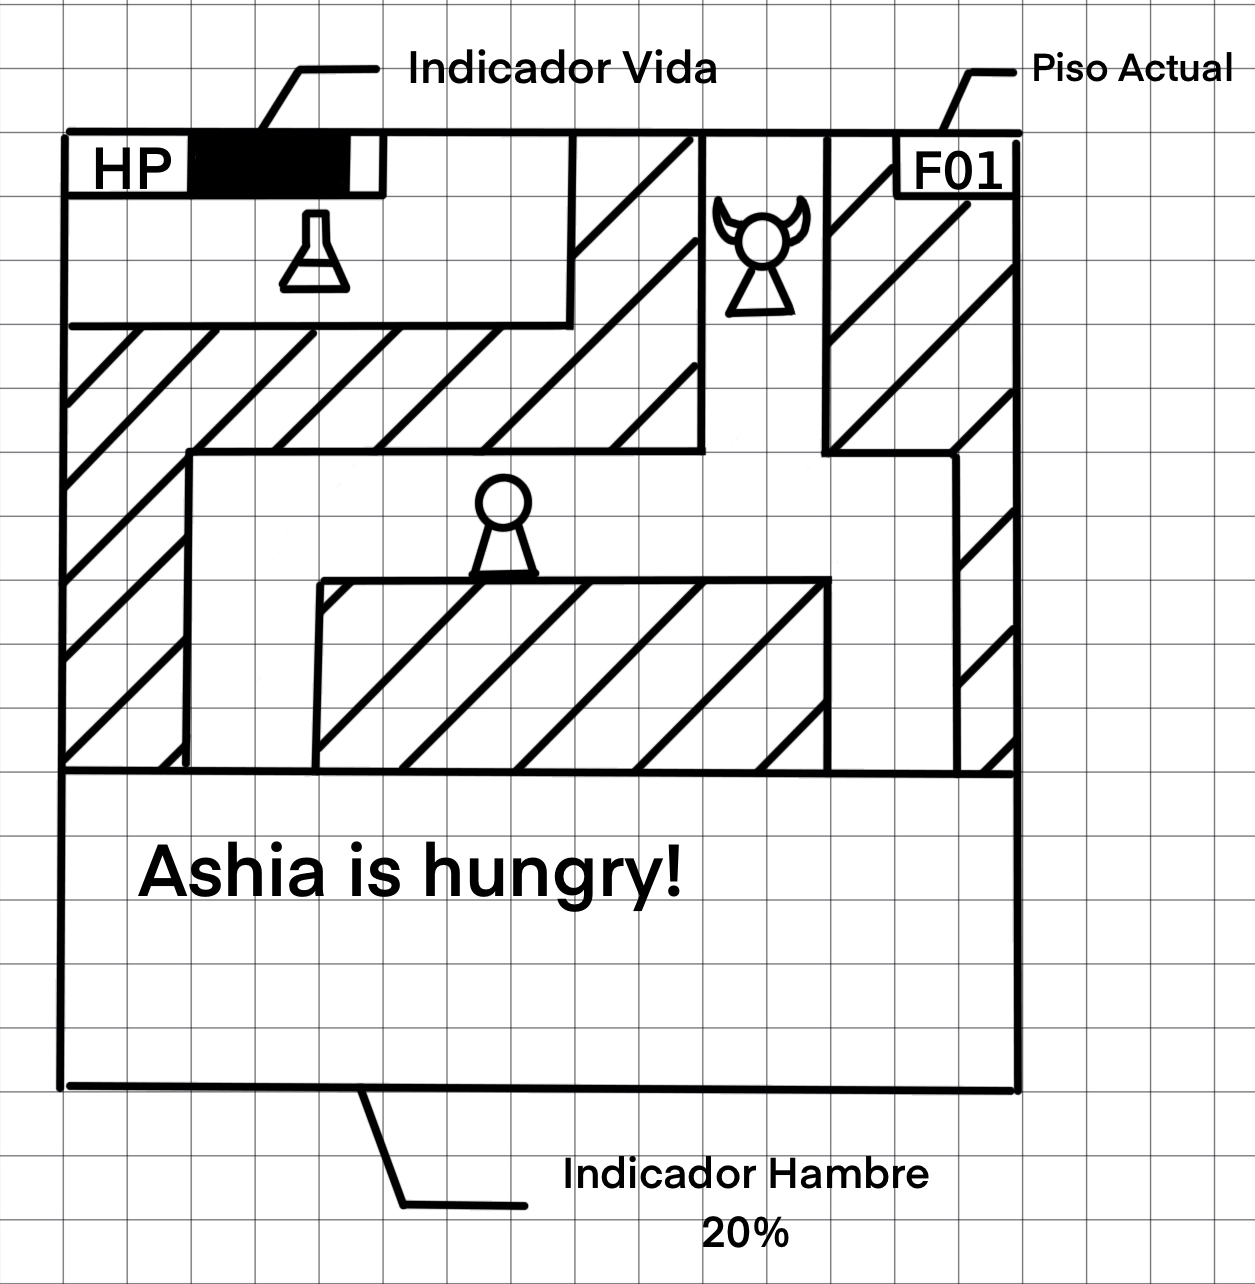
\includegraphics[width=0.5\textwidth]{include/images/gdd/gdd_hungry.png}
\caption{Mockup - Feedback de Hambre}
\label{figure:protagonist}
\end{figure}

Cuando se elimine a un enemigo, el jugador obtendrá \textbf{experiencia}. Con ella, podrá \textbf{subir de nivel} y \textbf{aumentar sus estadísticas base}. Por otro lado, gracias a unos \textbf{coleccionables}, podrá \textbf{mejorar el equipamiento y las armas que porte}.

\section{Personajes}

\subsection{Protagonista}

Nuestra protagonista, \textbf{Ashia}, será el \textbf{personaje que controle en todo momento el jugador}. Conforme avance en los niveles y consiga nuevo equipo, podrá recibir mejoras que la ayuden a enfrentarse a los enemigos.
\\ \\
Se realizó, tras varias opciones en formato tradicional, un \textbf{diseño completo del personaje} en formato digital. El resultado es el siguiente:

\begin{figure}[h]
\centering
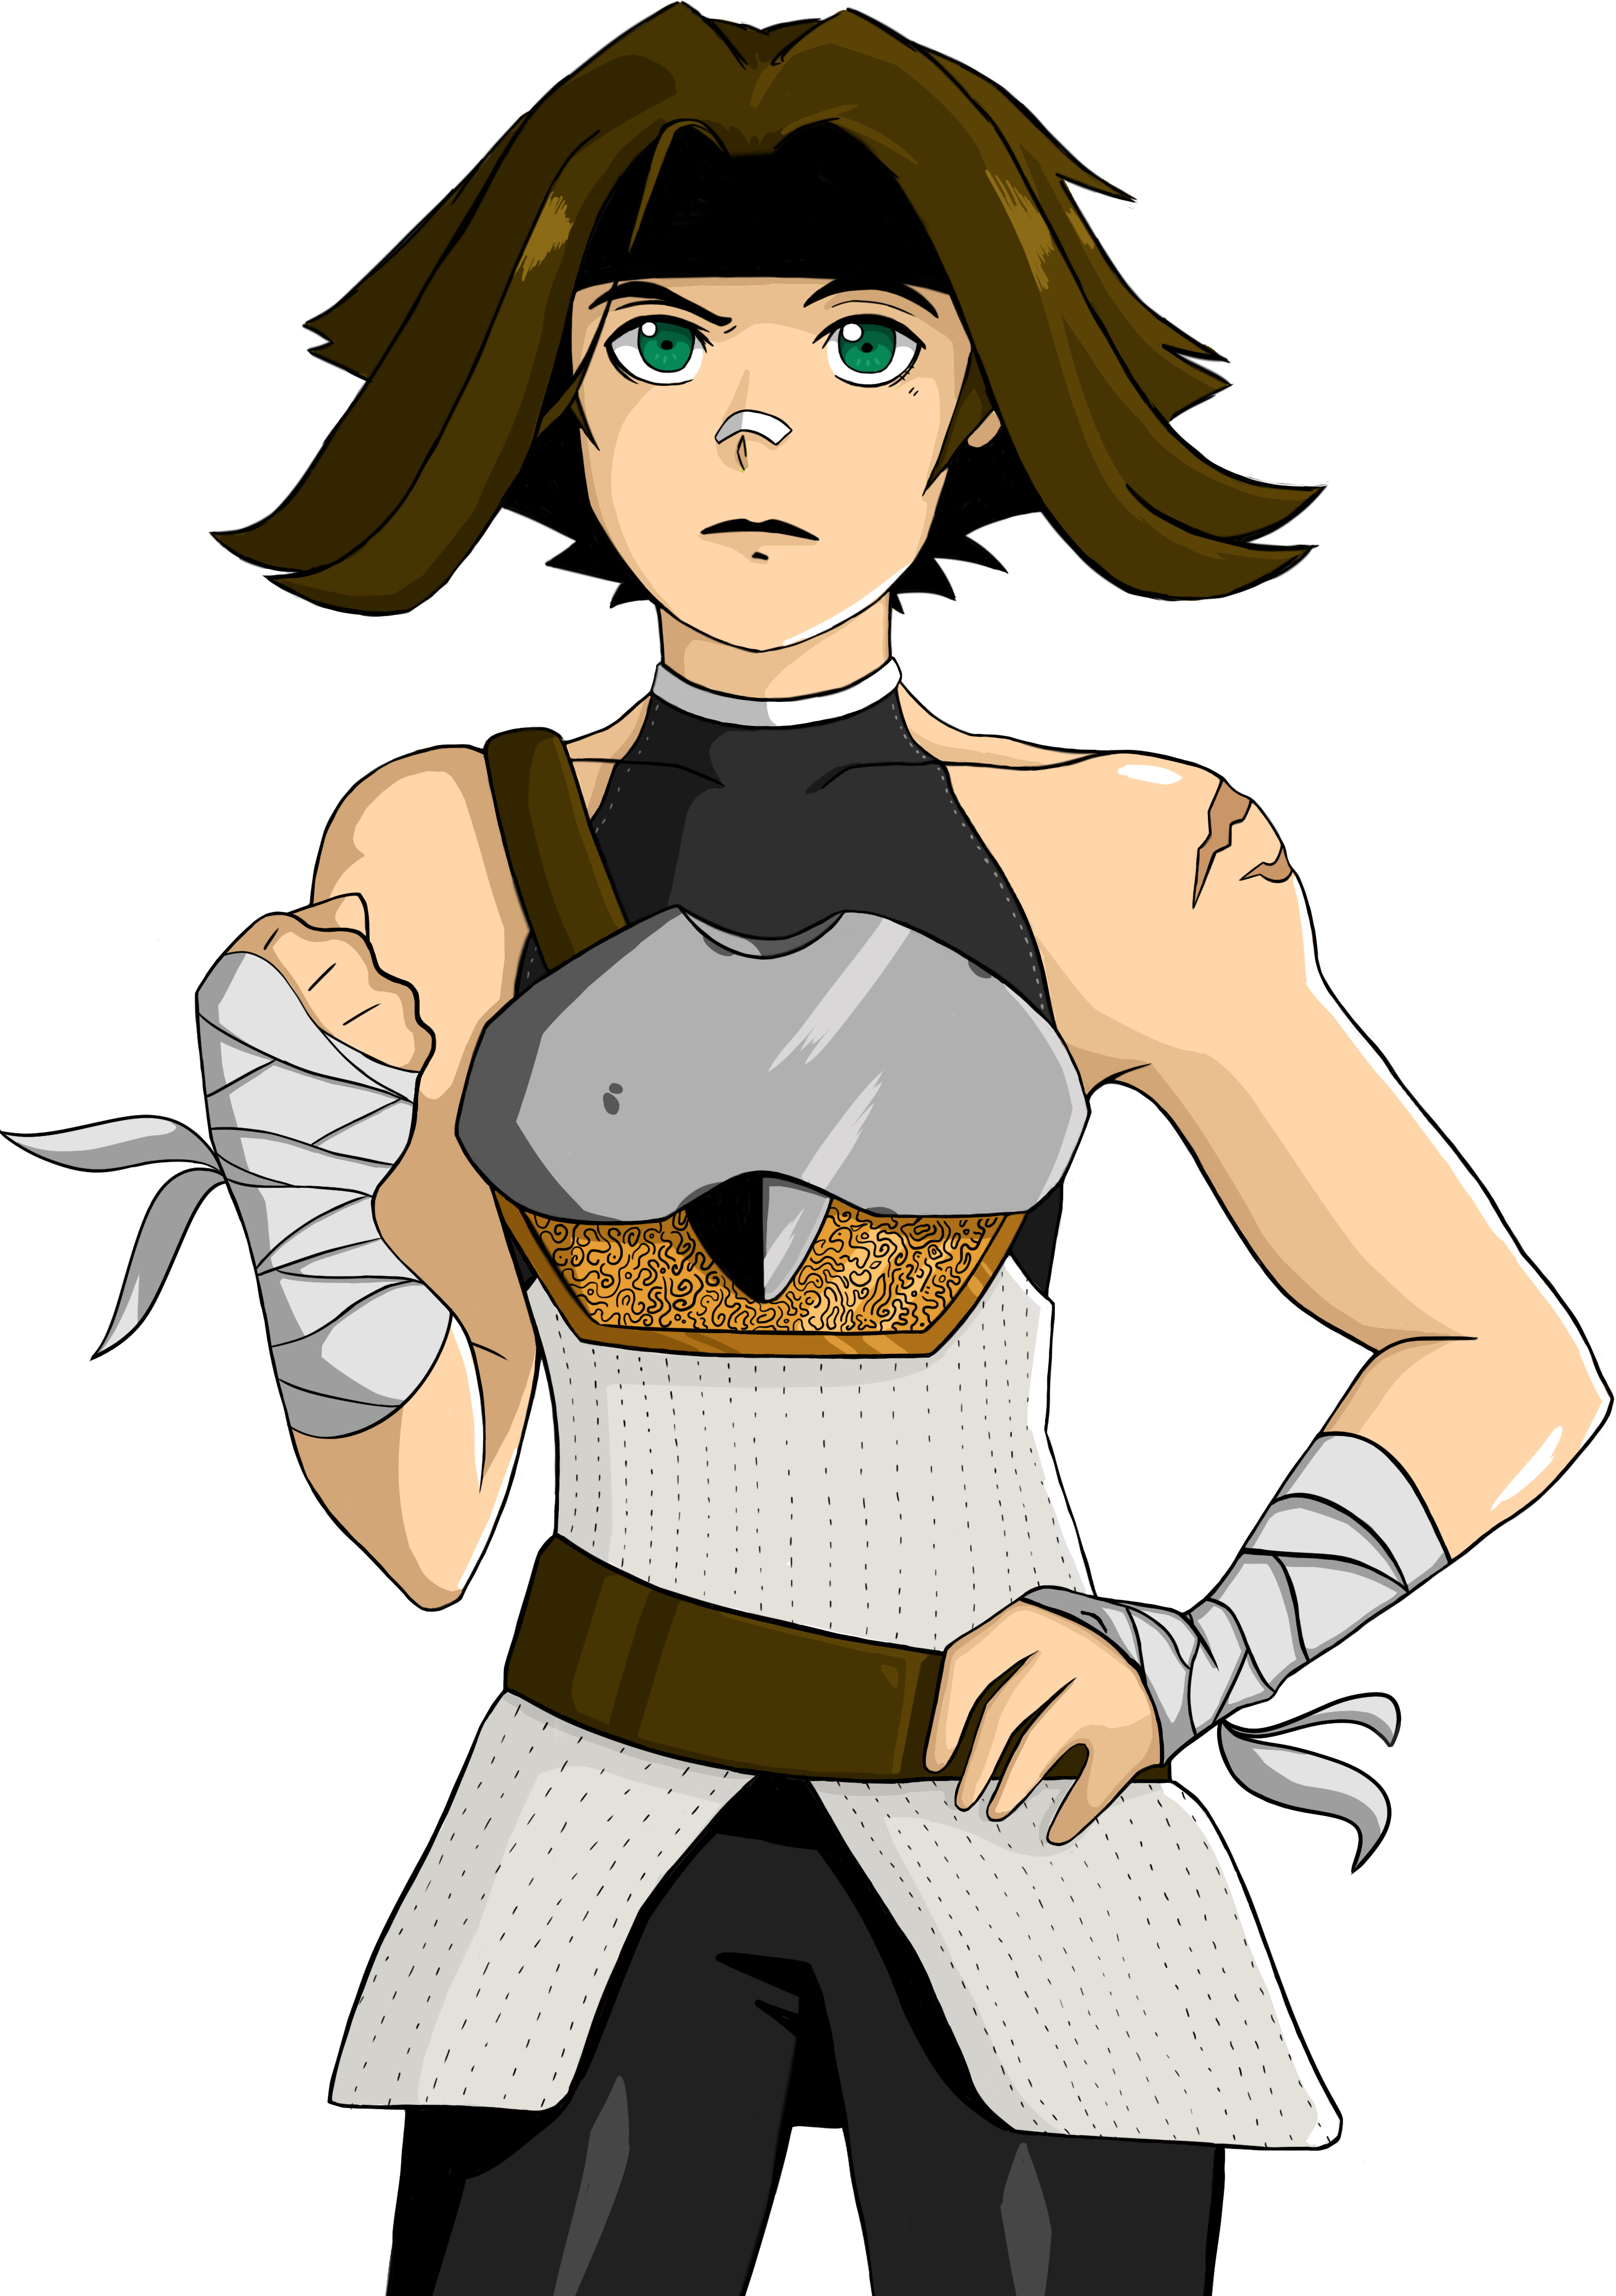
\includegraphics[width=0.5\textwidth]{include/images/desarrollo/protagonist.png}
\caption{Diseño de la Protagonista}
\label{figure:protagonist}
\end{figure}

Los sprites, al tener que ser de 4x4 tiles, pierden bastantes detalles en comparación a la fuente original. Sin embargo, captan perfectamente la esencia del personaje. A la hora de hacerlo, hubo una \textbf{inspiración importante} por parte de los sprites originales de las \textbf{entregas Pokémon Rojo/Azul}.

\clearpage

\begin{figure}[h]
\centering
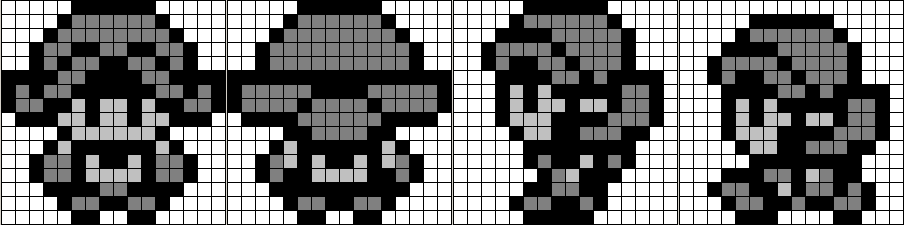
\includegraphics[width=0.7\textwidth]{include/images/gdd/gdd_protagonist.png}
\caption{Diseño los Sprites de la Protagonista}
\label{figure:protagonist_sprites}
\end{figure}

\subsection{Enemigos}

En cuanto a los \textbf{enemigos}, los vamos a dividir esencialmente en \textbf{dos apartados}: los enemigos \textbf{básicos} que vayan apareciendo en los niveles y el \textbf{jefe final}, el cual encontraremos llegados al piso más profundo de cada mazmorra.

\subsubsection{Básicos}

Todos los enemigos básicos poseerán la \textbf{misma inteligencia artificial}. Se \textbf{distinguirán} esencialmente por sus \textbf{sprites y estadísticas} (vida, resistencia, fuerza, etc.).
\\ \\
En la mayoría de casos su \textbf{comportamiento} se basará en intentar \textbf{atrapar al jugador y debilitarlo}. Podrán obtener, sin embargo, estados en los que sientan la necesidad de huir o utilizar algún objeto.
\\ \\
Los enemigos van a ser los siguientes:

\begin{itemize}
	\item \textbf{Enemigo Ladrón:} El enemigo más débil, pero de los más resistentes. Tiene 5 puntos de vida, 1 de velocidad y 5 de daño.
	\item \textbf{Enemigo Esqueleto:} El enemigo que más nos vamos a encontrar. Tiene 3 puntos de vida, 3/4 de velocidad y 10 de daño.
	\item \textbf{Enemigo Orco:} Un enemigo más feroz que el Esqueleto, con 3 puntos de vida, 2/3 de velocidad y 15 de daño.
	\item \textbf{Enemigo Armado:} El enemigo más poderoso de los 4, con 5 puntos de vida, 1/2 de velocidad y 15 de daño.
\end{itemize}

\begin{figure}[h]
\centering
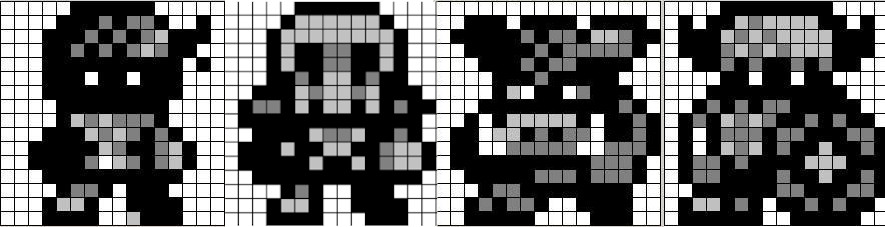
\includegraphics[width=0.7\textwidth]{include/images/desarrollo/allenemies.jpg}
\caption{Enemigos Base}
\label{figure:allenemies}
\end{figure}

\clearpage

\subsubsection{Jefe}

El \textbf{jefe} se halla en el \textbf{piso final de la mazmorra}. Ocupa el doble de casillas que cualquier enemigo básico y sus estadísticas son mucho mayores que las que pueda llegar a tener cualquier enemigo básico. Para derrotarlo, será esencial el uso de objetos que vaya encontrando por el camino o, por el contrario, tener el nivel necesario como para no necesitar el uso de estos.
\\ \\
La sala en la que se encuentran dista mucho del resto de pisos. En este caso no encontraremos ningunas escaleras u objetos. Será un área cuadrada, en el que solamente se encontrará el protagonista frente a frente con el enemigo.
\\ \\
El sprite que lo forma será de 4x4 tiles, a diferencia del jugador, compuesto de 2x2 tiles. Esto además, quiere decir que el rango de ataque del enemigo es mayor, como se muestra a continuación en el mockup:

\begin{figure}[h]
\centering
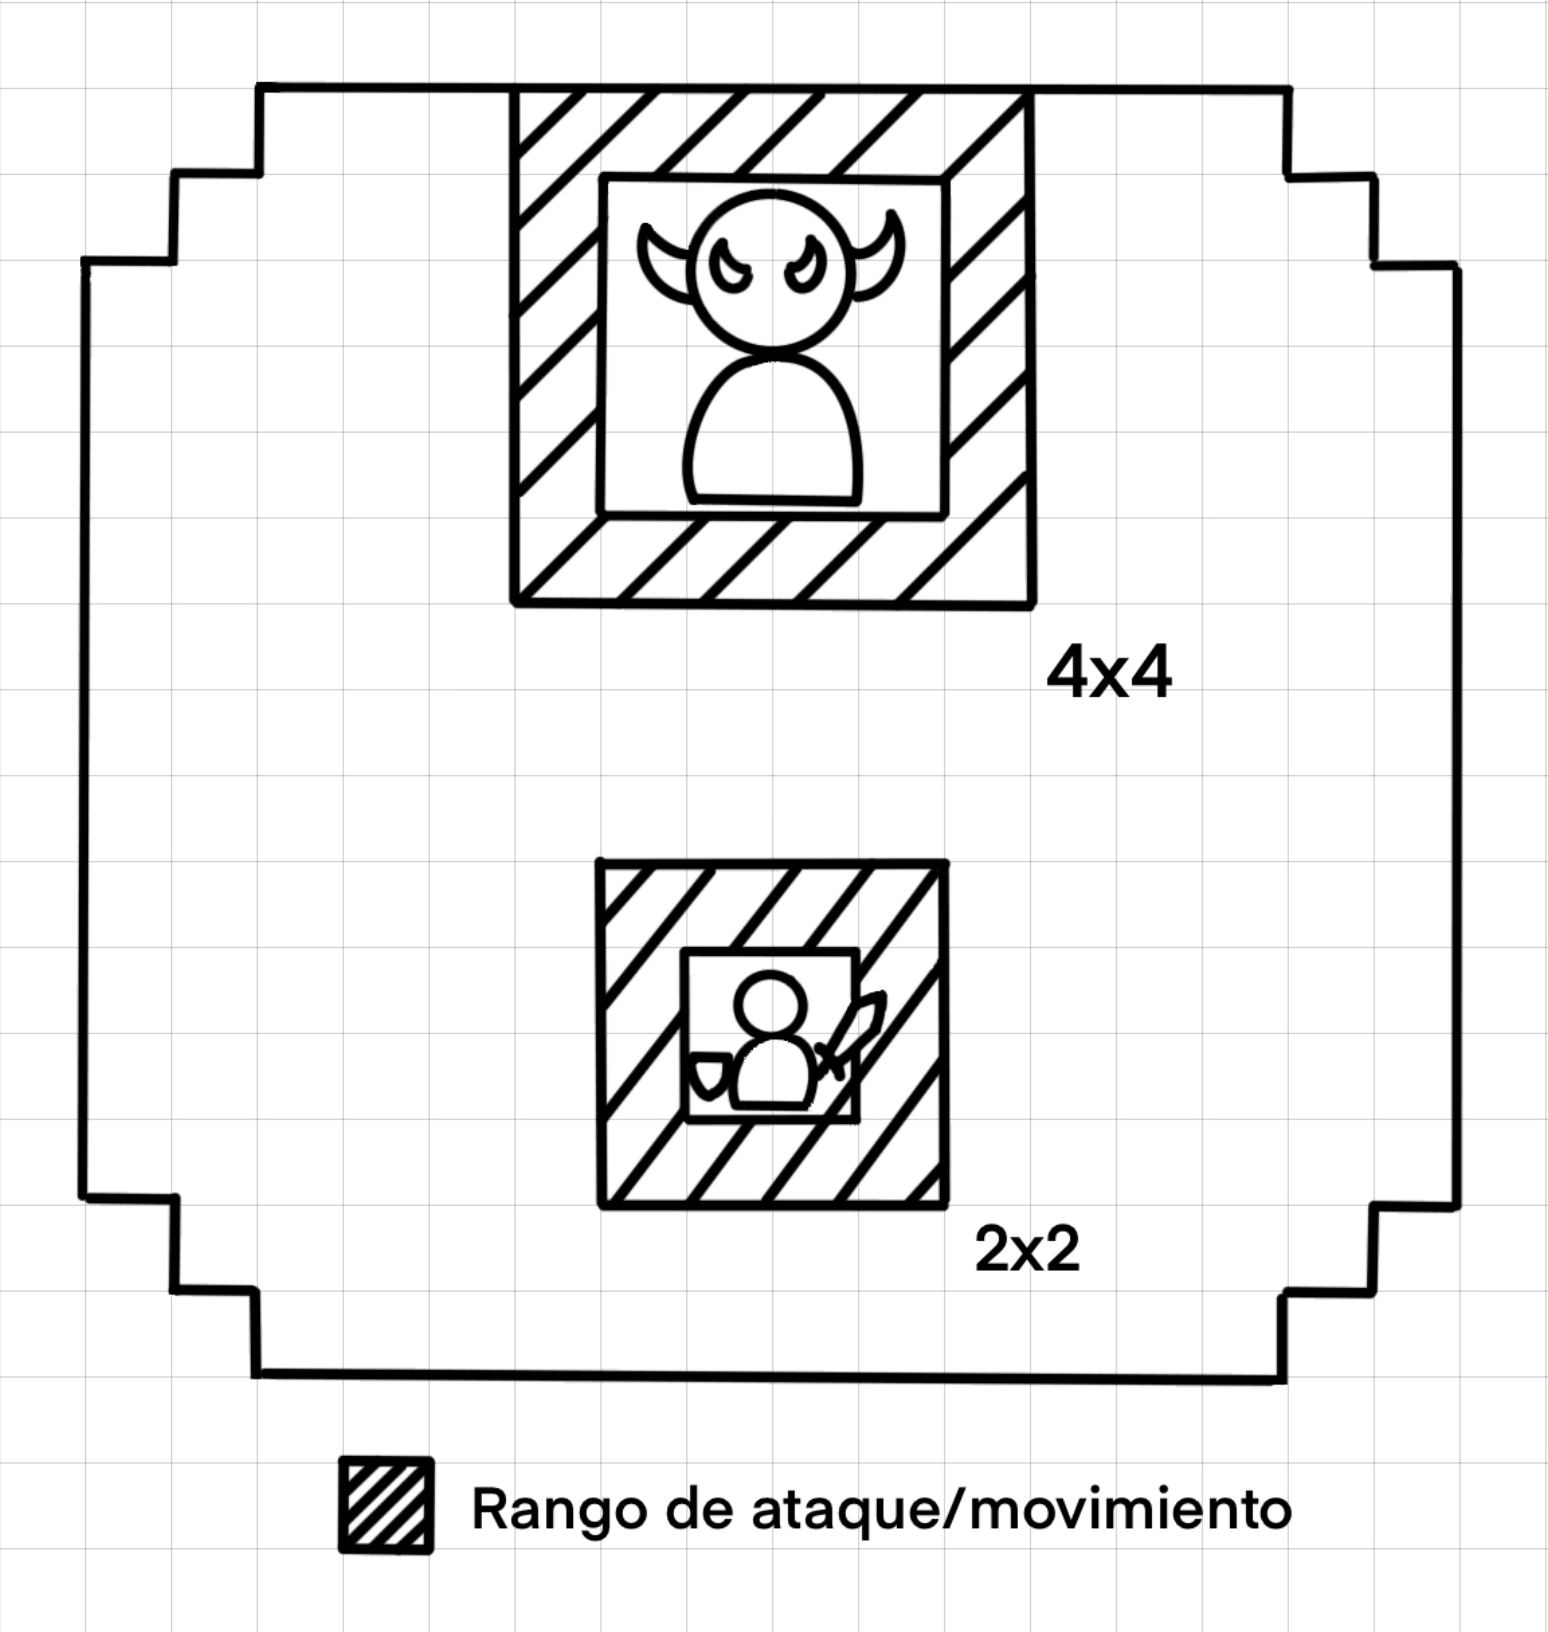
\includegraphics[width=0.5\textwidth]{include/images/gdd/gdd_boss.png}
\caption{Mockup - Diseño de Enemigo Jefe}
\label{figure:protagonist}
\end{figure}

\clearpage

\section{Controles}

Los controles de la Game Boy son muy sencillos y fáciles de entender. Lo único que vamos a tener que hacer es diferencias entre los dos estados del juego (mapa de mundo y mazmorras), ya que dependiendo de en la que el jugador se halle, deberemos activar o desactivar mecánicas como la de atacar o el consumo de turnos.

\subsection{Mapa de Mundo}

Vamos a definir el Mapa de Mundo como todas aquellas zonas por las que el jugador pueda moverse libremente y no hayan enemigos.

\begin{figure}[h]
\centering
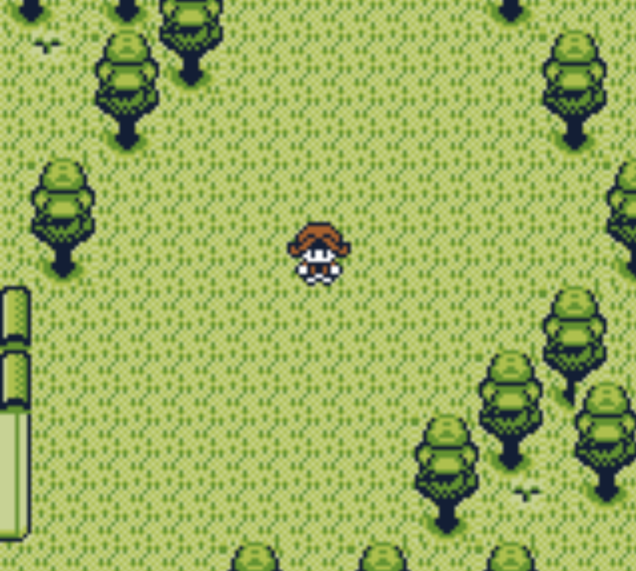
\includegraphics[width=0.5\textwidth]{include/images/gdd/overworld.png}
\caption{Mapa de Mundo}
\label{figure:overworld}
\end{figure}

Los controles van a ser los siguientes:

\begin{itemize}
	\item \textbf{PAD:} Movimiento del personaje.
	\item \textbf{Botón A:} Interactuar con el entorno (personajes u objetos) y avanzar en los diálogos.
	\item \textbf{Botón Start:} Acceso al menú de juego.
	\item \textbf{Botón Select:} Acceso a la vista del mapa del mundo.
\end{itemize}

\clearpage

\subsection{Mazmorras}

Accederemos a las mazmorras a través de distintas puertas localizadas en zonas concretas del mapa de mundo.

\begin{figure}[h]
\centering
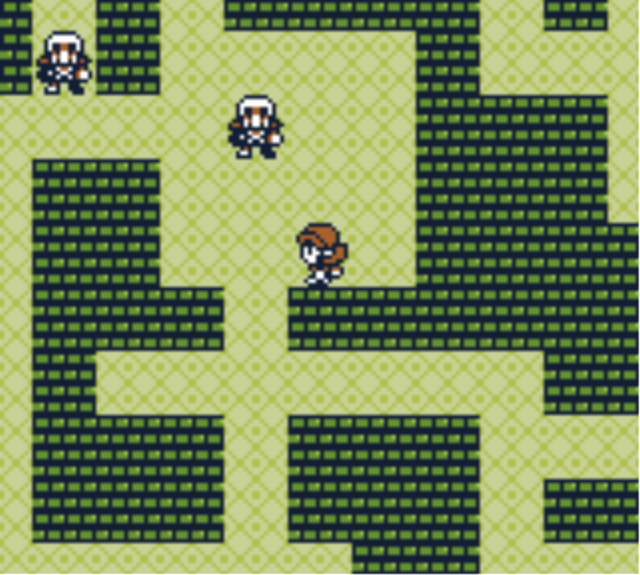
\includegraphics[width=0.5\textwidth]{include/images/gdd/dungeon.png}
\caption{Mazmorras}
\label{figure:dungeon}
\end{figure}

Los controles serán los mostrados a continuación:

\begin{itemize}
	\item \textbf{PAD:} Movimiento del personaje.
	\item \textbf{Botón A:} Avanzar en los diálogos.
	\item \textbf{Botón B:} Atacar.
	\item \textbf{Botón Start:} Acceso al menú de juego.
	\item \textbf{Botón Select:} Abrir mapa de la mazmorra.
\end{itemize}

\subsection{Menús}

Para el sistema de menús, los principales botones serán el A (aceptar) y el B (denegar). También se podrá salir inmediatamente (salvo algún caso específico) utilizando el botón Start.

\clearpage

\section{Pantallas}

A continuación se van a mostrar una serie de \textit{mockups} de los diferentes estados de juego en los que se puede encontrar el jugador.
\\ \\
La pantalla de título es el estado principal con el que comienza el videojuego cada vez que se encienda la consola. Se indicará la tecla que se debe pulsar para poder dar comienzo y simplemente se mostrará un fondo con algún dibujo, el título por encima de este y el nombre del autor junto a la fecha de creación.

\begin{figure}[h]
\centering
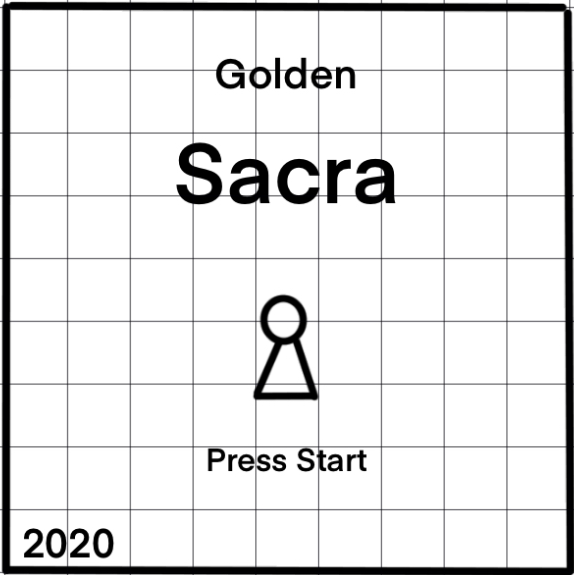
\includegraphics[width=0.4\textwidth]{include/images/gdd/gdd_title.png}
\caption{Mockup - Pantalla de Título}
\label{figure:gddtitle}
\end{figure}

El segundo estado, inmediatamente después de la pantalla de título, es la del mapa del mundo. Aquí el jugador va a poder explorar un poco la zona, hablar con distintos NPC's y decidir a qué localizaciones acceder (viviendas o mazmorras).

\begin{figure}[h]
\centering
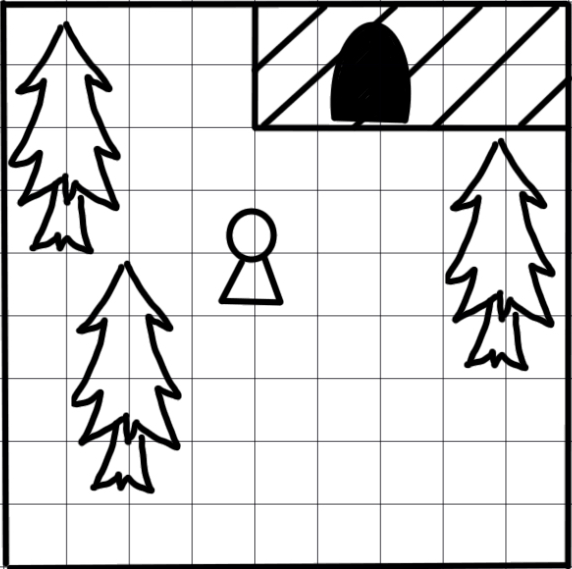
\includegraphics[width=0.4\textwidth]{include/images/gdd/gdd_overworld.png}
\caption{Mockup - Diseño de Mapa de Mundo}
\label{figure:gddoverworld}
\end{figure}

Las viviendas se compondrán principalmente de uno o varios NPC's con los que poder interaccionar y diversos muebles que decorarán el interior. En alguna ocasión, el jugador encontrará objetos escondidos en estos sitios que le serán de ayuda en su aventura. También existirá la posibilidad de comprar objetos a un mercader el cual se podrá encontrar en una de estas zonas.

\begin{figure}[h]
\centering
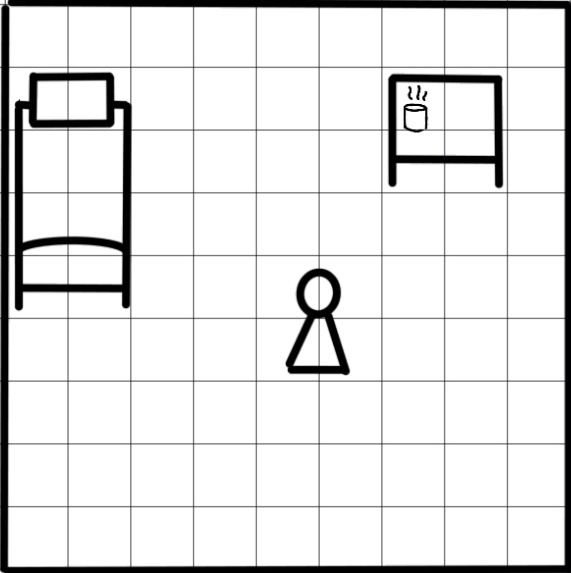
\includegraphics[width=0.4\textwidth]{include/images/gdd/gdd_house.png}
\caption{Mockup - Diseño de Vivienda}
\label{figure:gddhouse}
\end{figure}

Otra pantalla será la del menú y la del inventario. A esta segunda podremos acceder a través de la primera, además de guardar la partida. El inventario mostrará todos los objetos y las cantidades de las que se disponen en ese momento.

\begin{figure}[h]
\centering
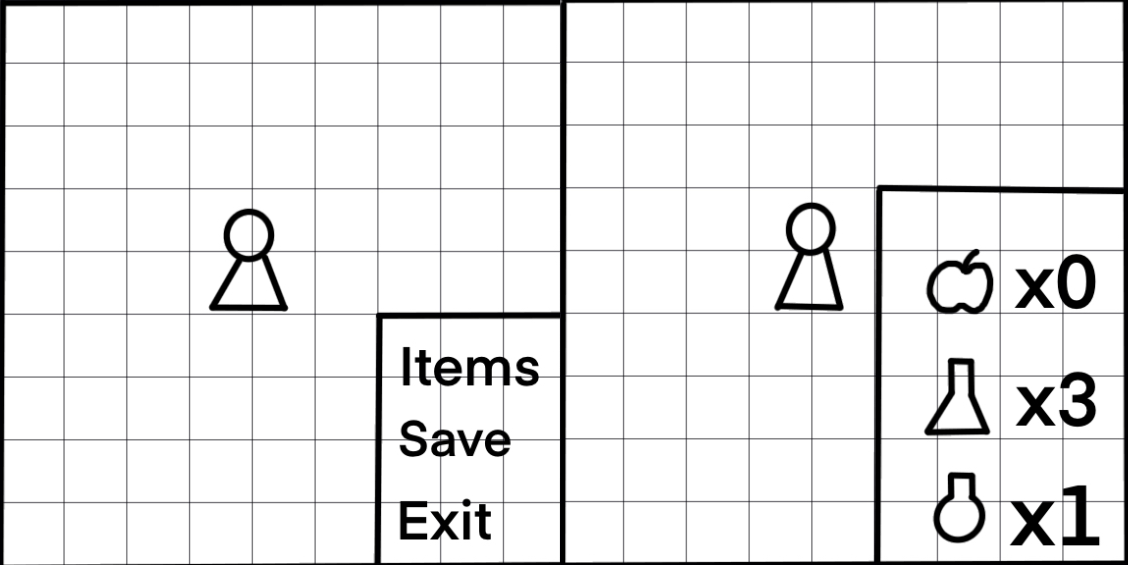
\includegraphics[width=0.7\textwidth]{include/images/gdd/gdd_menu.png}
\caption{Mockup - Diseño de Menú e Inventario}
\label{figure:gddmenuinv}
\end{figure}

\clearpage

\section{Estados de Juego}

Vamos a ver cómo se relacionan entre sí todos los estados del juego mediante un diagrama de flujo. Esto es útil para que sepamos, a la hora de programar, desde qué estados se puede o debe acceder a otro.

\begin{figure}[h]
\centering
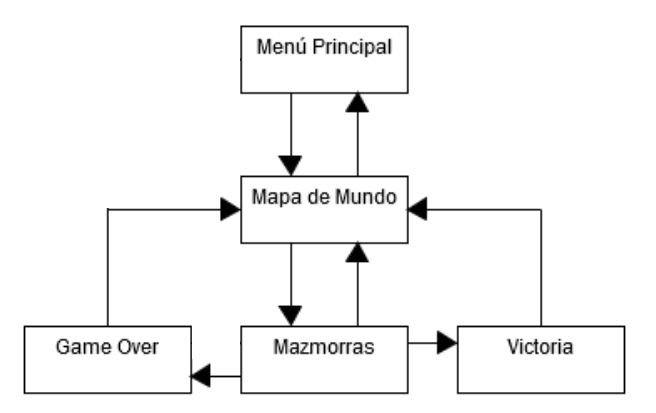
\includegraphics[width=0.7\textwidth]{include/images/gdd/flow.png}
\caption{Diagrama de Flujo}
\label{figure:gddflow}
\end{figure}

Como ya se ha comentado, el primer estado es el de pantalla de título. Desde aquí solamente podremos acceder al estado de mapa de mundo, en el cual el jugador podrá decidir explorar o adentrarse en las mazmorras. Una vez aquí dentro, podremos volver al mapa del menú siempre que muramos o lleguemos al último piso de todos. Se podrá salir también desde la propia mazmorra guardando la partida, lo que provocará que se teletransporte el jugador a este estado.

\cleardoublepage


